\documentclass[11pt,a4paper]{article}
\usepackage[a4paper,margin=1in]{geometry}
\usepackage{amsmath,amssymb,amsthm}
\usepackage{graphicx}
\usepackage{booktabs}
\usepackage{caption}
\usepackage{subcaption}
\usepackage{hyperref}
\usepackage{xcolor}
\hypersetup{colorlinks=true, linkcolor=blue!60!black, citecolor=blue!60!black, urlcolor=blue!60!black}
\usepackage{enumitem}
\usepackage{multicol}
\usepackage{authblk}
\usepackage{natbib}
\bibliographystyle{plainnat}
\setlength{\bibsep}{2pt}

\graphicspath{{../figures/}}

\title{\textbf{Modelling the Six Size--Value Portfolios and Designing Trading Strategies on the Kenneth French Data Library (Jul.\ 1926 -- Jan.\ 2026)}}
\author{FMA4200 Financial Data Analysis: Final Project}
\date{16 May 2026}

\begin{document}
\maketitle

\begin{abstract}
\noindent We study the monthly value-weighted returns of the six size--book-to-market portfolios from Kenneth French's Data Library over a 99.6-year sample. We characterise the distributional properties, fit a sequence of linear and conditional-heteroskedasticity time-series models, and use Fama--French style factor proxies as exogenous predictors. We then turn to portfolio construction: we examine multivariate dependence and pairwise cointegration, estimate the unconditional mean--variance frontier, and benchmark a battery of allocation rules out-of-sample. The plug-in mean--variance strategy collapses under estimation error (annualised Sharpe of 0.02 with extreme leverage), while a long-only re-formulation combined with Ledoit--Wolf covariance shrinkage achieves a Sharpe of 0.69 and dominates the equally-weighted benchmark on a risk-adjusted basis. The global minimum-variance portfolio is the single best-performing rule (Sharpe = 0.76), confirming the well-known empirical superiority of strategies that rely on covariance information only.
\end{abstract}

\section{Introduction}

\subsection{Motivation and background}
The cross-section of U.S.\ equity returns has been organised along the size and book-to-market dimensions since the seminal work of \citet{FamaFrench1992,FamaFrench1993}. Kenneth French's Data Library makes the six benchmark size $\times$ book-to-market portfolios publicly available at the monthly frequency back to July 1926, providing one of the longest continuous return series in academic finance. These portfolios are the canonical inputs for tests of asset pricing models, for assessing factor risk premia, and for evaluating active strategies. The present study uses them simultaneously as (i) test assets for time-series modelling of returns and volatility and (ii) building blocks for systematic portfolio construction. The motivation is twofold. First, the size and value tilts are widely viewed as compensated risk premia and a careful description of their conditional and unconditional distributions is a prerequisite for any inference, backtest, or risk-budget exercise. Second, a near-century of data lets us evaluate trading strategies through multiple regimes, including the Great Depression, the post-war expansion, the inflationary 1970s, the tech bubble, the global financial crisis, the COVID shock, and the post-2022 rate cycle.

\subsection{Literature review}
The time-series modelling of equity returns rests on three pillars.\footnote{We follow the textbook treatments of \citet{Tsay2010} and \citet{HamiltonTS} throughout.} \emph{(i) Distributional features.} Mean monthly returns are positive and small relative to their standard deviation; the distribution is leptokurtic and frequently skewed, well documented since \citet{FamaFat1965} and \citet{Mandelbrot1963}. \emph{(ii) Linear dependence.} Although individual stock returns are close to a martingale difference, monthly portfolio returns exhibit modest predictability from past returns, dividend yields, and macro factors \citep{CampbellShiller1988,KeimStambaugh1986,WelchGoyal2008}. Autoregressive moving-average (ARMA) models, often differenced to ARIMA when prices rather than returns are studied, provide a parsimonious description of the conditional mean. \emph{(iii) Conditional variance.} Volatility is persistent and clustered; the ARCH model of \citet{Engle1982} and its GARCH generalisation \citep{Bollerslev1986} are the standard workhorses. We add Fama--French style exogenous regressors to obtain ARIMAX/ARMA-X benchmarks.

For trading strategies the literature has two complementary strands. The \emph{cointegration} branch \citep{EngleGranger1987,Johansen1991} underlies statistical-arbitrage pairs trading \citep{GatevGoetzmannRouwenhorst2006,Krauss2017}: long-run equilibria between asset pairs identify mean-reverting spreads that can be traded with stop-loss rules. The \emph{Markowitz} branch \citep{Markowitz1952,SharpeCAPM,JagannathanMa2003} forms portfolios from estimated means and covariance matrices. A robust empirical finding, formalised by \citet{DeMiguelGarlappiUppal2009}, is that the plug-in mean--variance strategy underperforms the equally-weighted (1/$N$) benchmark out-of-sample because of estimation error in the sample mean. Two large families of fixes have been studied: \emph{shrinkage} of $\hat{\Sigma}$ \citep{LedoitWolf2004} and of $\hat{\mu}$ \citep{Jorion1986}; and constrained optimisation, including no-short-sale constraints \citep{JagannathanMa2003} and risk-parity weightings \citep{Maillard2010}.

\subsection{Contributions and key findings}
This project is fundamentally a quantitative case study that bridges the modelling and the asset-allocation literatures. Our specific contributions are as follows. First, we provide a unified description of the unconditional moments, autocorrelation structure, conditional heteroskedasticity, and stationarity of all six portfolios over the full sample. Returns are highly non-normal (Jarque--Bera $p$-values $<10^{-200}$ for all six series) and stationary at every conventional level; ARCH effects are extreme. Second, we fit best-BIC ARMA models per portfolio and show that they remove the linear dependence in the residuals but leave overwhelming evidence of conditional heteroskedasticity, which a GARCH(1,1) layer absorbs cleanly (Ljung--Box $p$-values on squared standardised residuals all $> 0.5$). Third, we incorporate Fama--French exogenous variables. Their explanatory power in a contemporaneous factor regression is large ($R^2 \in [0.86, 0.97]$), but lagged versions cannot beat naive forecasts out-of-sample (negative OOS $R^2$ for all six portfolios), consistent with the limits-of-predictability literature \citep{WelchGoyal2008}. Fourth, we conduct an Engle--Granger cointegration screen across the 15 pairs, find weak evidence (only one pair passing at 5\%), and show that a z-score-based pairs trade on the strongest pair fails to deliver a positive Sharpe ratio: the apparent long-run equilibrium is too noisy and too non-stationary to support a profitable strategy at the monthly frequency. Fifth, we map out the unconditional mean--variance frontier and run a walk-forward backtest of six allocation rules. The unconstrained plug-in tangency portfolio behaves pathologically (annualised volatility $\approx 438\%$, Sharpe $\approx 0$); both Ledoit--Wolf shrinkage applied to a long-only re-formulation and the global minimum-variance portfolio dominate the equally-weighted benchmark on a risk-adjusted basis. The clear ordering of strategies by Sharpe ratio is GMV $>$ Long-only-Tangency $\approx$ Long-only-Shrinkage $>$ Risk-Parity $>$ Equal-Weighted $\gg$ Plug-in Tangency, in line with \citet{DeMiguelGarlappiUppal2009} and \citet{JagannathanMa2003}.

\section{Data Source and Processing}

\subsection{Data source}
The data are taken from Kenneth French's \emph{6 Portfolios Formed on Size and Book-to-Market (2 $\times$ 3)} file from the Data Library on Tuck's website. We use the value-weighted monthly returns, which span $T=1{,}195$ months from July 1926 through January 2026. Portfolios are formed at the end of each June by sorting NYSE/AMEX/Nasdaq common stocks into two market-cap groups (SMALL, BIG) and three book-to-market groups (LoBM = growth, BM2 = neutral, HiBM = value), giving six portfolios:
\[
\text{SMALL.LoBM},\quad \text{ME1.BM2},\quad \text{SMALL.HiBM},\quad \text{BIG.LoBM},\quad \text{ME2.BM2},\quad \text{BIG.HiBM}.
\]

\subsection{Preprocessing}
The raw file contains 15 lines of metadata, monthly returns expressed as percentages, and footers including the annual block (which we discard). We read only the monthly value-weighted block, parse \texttt{YYYYMM} timestamps into month-end dates, coerce all return columns to floating point, and replace the sentinel codes $-99.99$ and $-999$ by missing values. After this filter no rows are dropped.

For the exogenous regressors required by the predictive modelling exercise we cannot fetch the Fama--French 3-factor file from the network in our environment, so we construct \emph{leave-one-out} (LOO) proxies internally. For each target portfolio $i$, the proxies use only the other five portfolios:
\begin{align}
\widehat{\text{Mkt}}_t^{(-i)} - r_f &= \tfrac{1}{5}\sum_{j \ne i} R_{j,t} - r_f,\\
\widehat{\text{SMB}}_t^{(-i)} &= \overline{R}_{\text{SMALL,-i,t}} - \overline{R}_{\text{BIG,-i,t}},\\
\widehat{\text{HML}}_t^{(-i)} &= \overline{R}_{\text{HiBM,-i,t}} - \overline{R}_{\text{LoBM,-i,t}},
\end{align}
where $r_f = 0.3\%$/month is a constant short-rate proxy. The LOO construction is essential: it prevents mechanical fit when the target appears on both sides of the regression. We additionally form a slow 12-month term-spread proxy as the difference between the BIG- and SMALL-stock moving averages.

\subsection{Variable summary}
Table~\ref{tab:descriptive} reports the unconditional moments, Jarque--Bera (JB) normality test, Ljung--Box on returns and squared returns ($Q(12)$ and $Q^2(12)$), Engle's ARCH-LM test at five lags, and the augmented Dickey--Fuller (ADF) statistic with constant. Figure~\ref{fig:ts} plots the six return series; Figure~\ref{fig:hist} overlays the empirical density with a fitted normal.

\begin{table}[h!]
\centering
\caption{Descriptive statistics for the monthly returns (percent). $p$-values in parentheses. JB: Jarque--Bera test of normality. $Q(12)$ and $Q^2(12)$: Ljung--Box on raw and squared returns. ARCH(5): Engle's LM test. ADF: ADF $t$-statistic with constant; the 1\%, 5\%, 10\% critical values are $-3.43, -2.86, -2.57$.}
\label{tab:descriptive}
\small
\begin{tabular}{lrrrrrrrrrr}
\toprule
Portfolio & Mean & SD & Skew & Ex.\ Kurt & JB & $Q(12)$ & $Q^2(12)$ & ARCH(5) & ADF & Lag \\
\midrule
SMALL.LoBM & 0.97 & 7.43 & 0.57 & 6.92 & 2451 & 44.0 & 435 & 162 & $-9.61$ & 12 \\
           &      &      &      &      & (0.000) & (0.000) & (0.000) & (0.000) & & \\
ME1.BM2    & 1.24 & 6.94 & 1.10 & 13.41 & 9192 & 75.7 & 670 & 195 & $-9.72$ & 12 \\
           &      &      &      &      & (0.000) & (0.000) & (0.000) & (0.000) & & \\
SMALL.HiBM & 1.42 & 8.08 & 1.96 & 20.85 & 22420 & 87.9 & 650 & 194 & $-9.37$ & 12 \\
           &      &      &      &      & (0.000) & (0.000) & (0.000) & (0.000) & & \\
BIG.LoBM   & 0.96 & 5.27 & $-0.13$ & 5.20 & 1351 & 24.1 & 477 & 120 & $-9.17$ & 12 \\
           &      &      &      &      & (0.000) & (0.020) & (0.000) & (0.000) & & \\
ME2.BM2    & 0.96 & 5.60 & 1.16 & 17.20 & 15000 & 66.3 & 845 & 196 & $-9.22$ & 12 \\
           &      &      &      &      & (0.000) & (0.000) & (0.000) & (0.000) & & \\
BIG.HiBM   & 1.21 & 7.08 & 1.44 & 17.45 & 15574 & 54.9 & 799 & 245 & $-9.33$ & 12 \\
           &      &      &      &      & (0.000) & (0.000) & (0.000) & (0.000) & & \\
\bottomrule
\end{tabular}
\end{table}

Three patterns dominate Table~\ref{tab:descriptive}. First, the historical \emph{size and value premia} are clearly visible: SMALL.HiBM (small-value) earns 1.42\% per month while BIG.LoBM (large-growth) earns only 0.96\%, a 46 bp/month spread or about 5.6\% per year. Second, the distributions are far from normal: skewness is positive and large for five of the six portfolios and excess kurtosis ranges from 5.2 (BIG.LoBM) to 20.9 (SMALL.HiBM); JB rejects normality at any conventional level. Third, every series exhibits strong autocorrelation in squared returns and rejects the no-ARCH null with $p$-values below $10^{-22}$. The ADF $t$-statistic is below $-9.0$ in every case, meaning unit-root non-stationarity is strongly rejected; the return series are stationary, as expected.

\begin{figure}[h!]
\centering
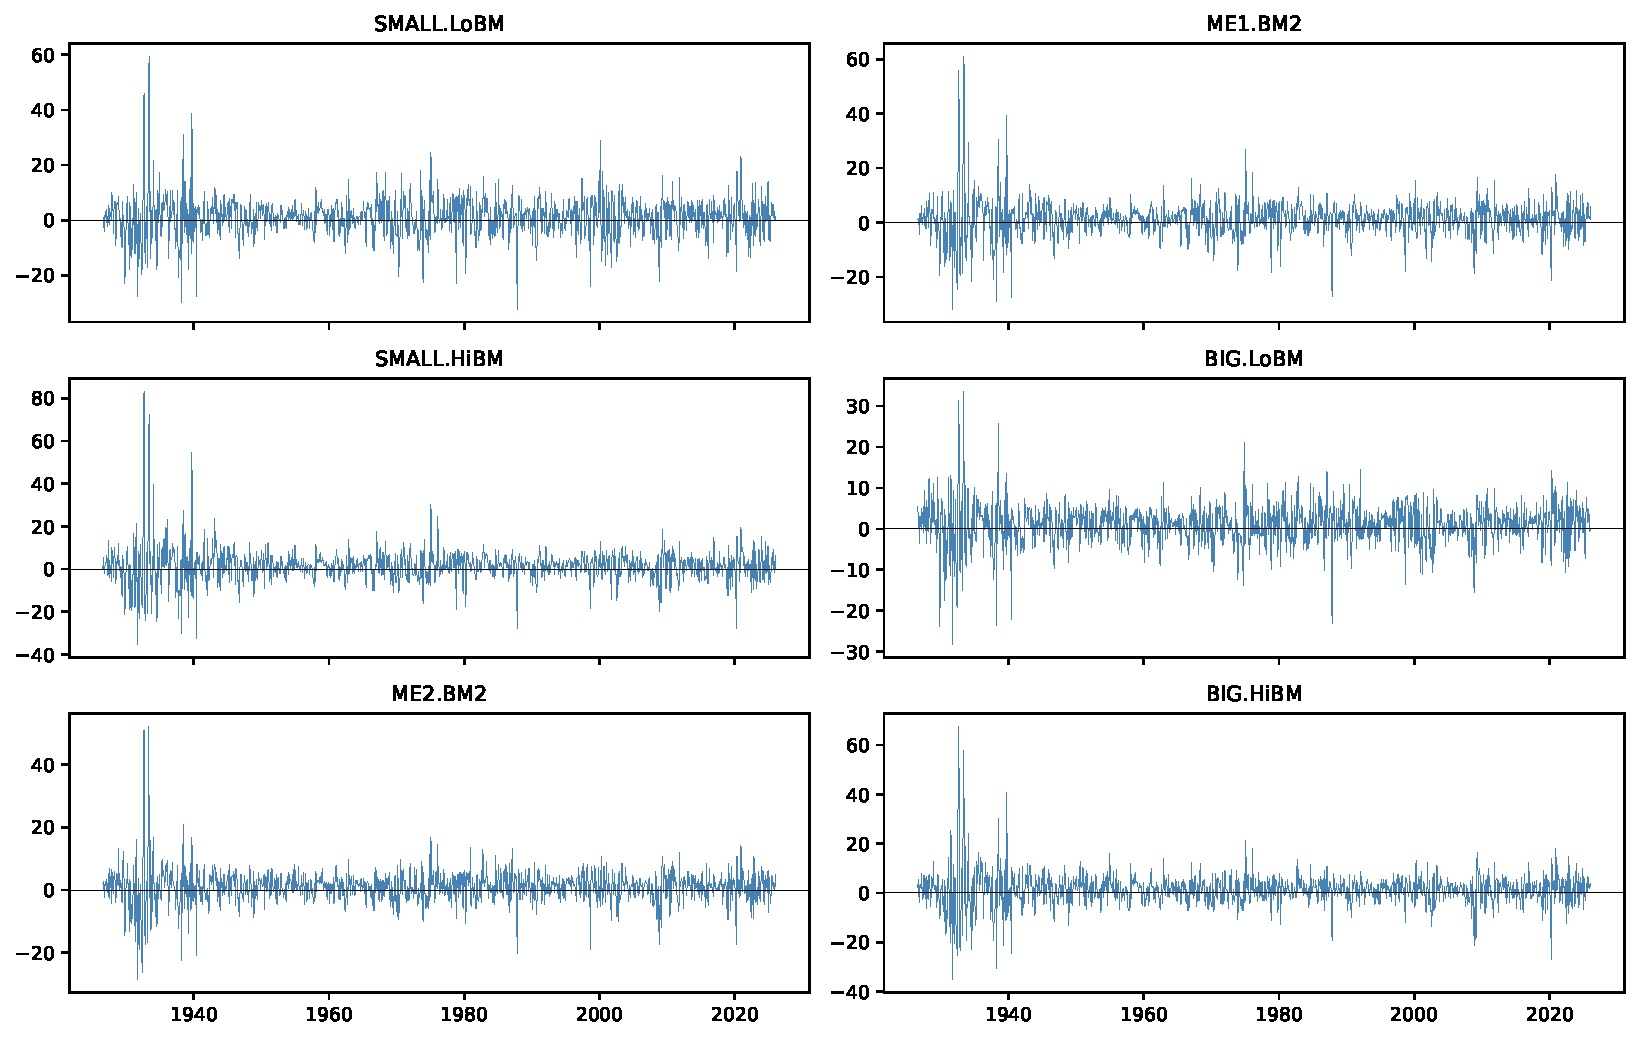
\includegraphics[width=\textwidth]{returns_timeseries.pdf}
\caption{Monthly returns (\%) for the six size $\times$ book-to-market portfolios, Jul.\ 1926 -- Jan.\ 2026. Periods of clustered volatility (1929--32, 1937, 1973--74, 1987, 2000--02, 2008--09, 2020) are visible in all panels.}
\label{fig:ts}
\end{figure}

\begin{figure}[h!]
\centering
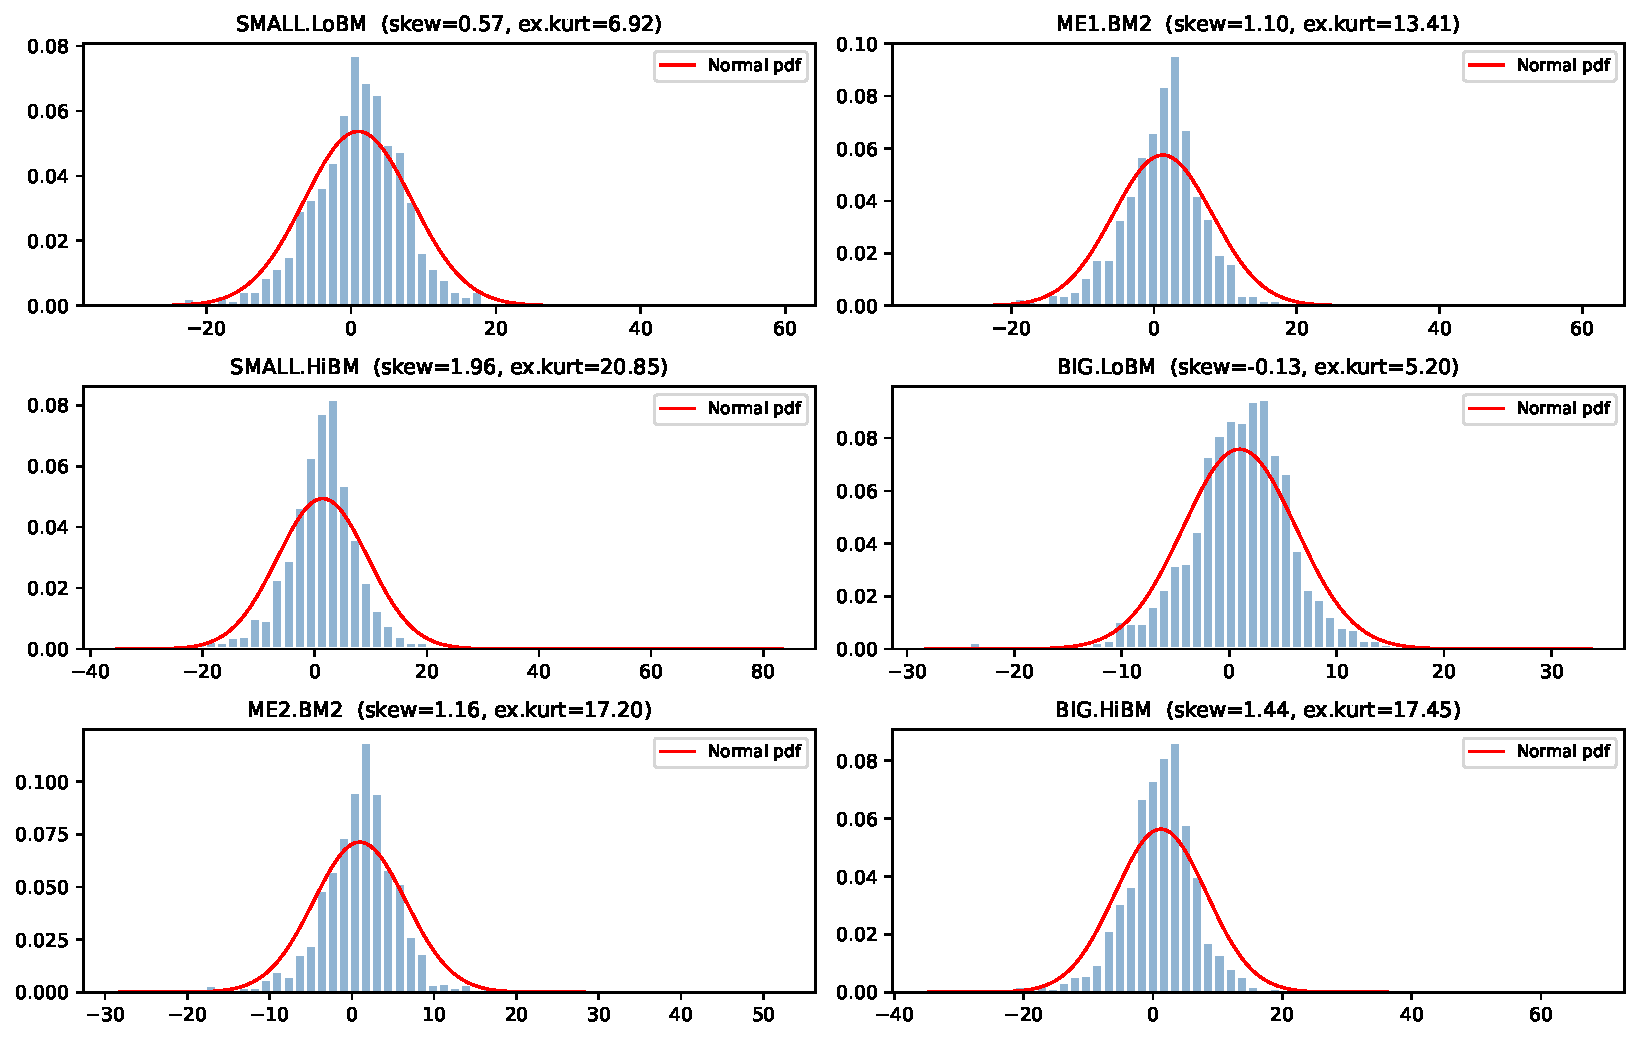
\includegraphics[width=\textwidth]{return_histograms.pdf}
\caption{Empirical density of monthly returns with a fitted Gaussian density in red. The fat right tails and excess peakedness relative to the normal are obvious in every panel.}
\label{fig:hist}
\end{figure}

\section{Modelling the Individual Portfolio Returns}

\subsection{Distributional properties}
The unconditional distributions are leptokurtic and right-skewed for the small-cap and value portfolios (the only exception is BIG.LoBM, which is mildly left-skewed). The right tail is driven by sharp rebounds (October 1974, January 1975 and April 2020 each produced two-digit returns for SMALL.HiBM). These features are consistent with the standard finding that a heavy-tailed unconditional distribution arises naturally from a model with conditionally Gaussian innovations and persistent volatility \citep{Bollerslev1986}, which we will exploit in the GARCH layer.

\subsection{Linear time-series modelling: AR, MA, ARMA, ARIMA}
Returns are stationary (Table~\ref{tab:descriptive}), so no differencing is required and ARIMA collapses to ARMA. Figure~\ref{fig:acf} shows that the autocorrelation function dies out quickly while the partial autocorrelation function has a few significant low-order lags. We search over $\text{ARMA}(p,q)$ with $p, q \le 2$ and select by Schwarz's BIC. The selected orders are reported in Table~\ref{tab:arma}.

\begin{figure}[h!]
\centering
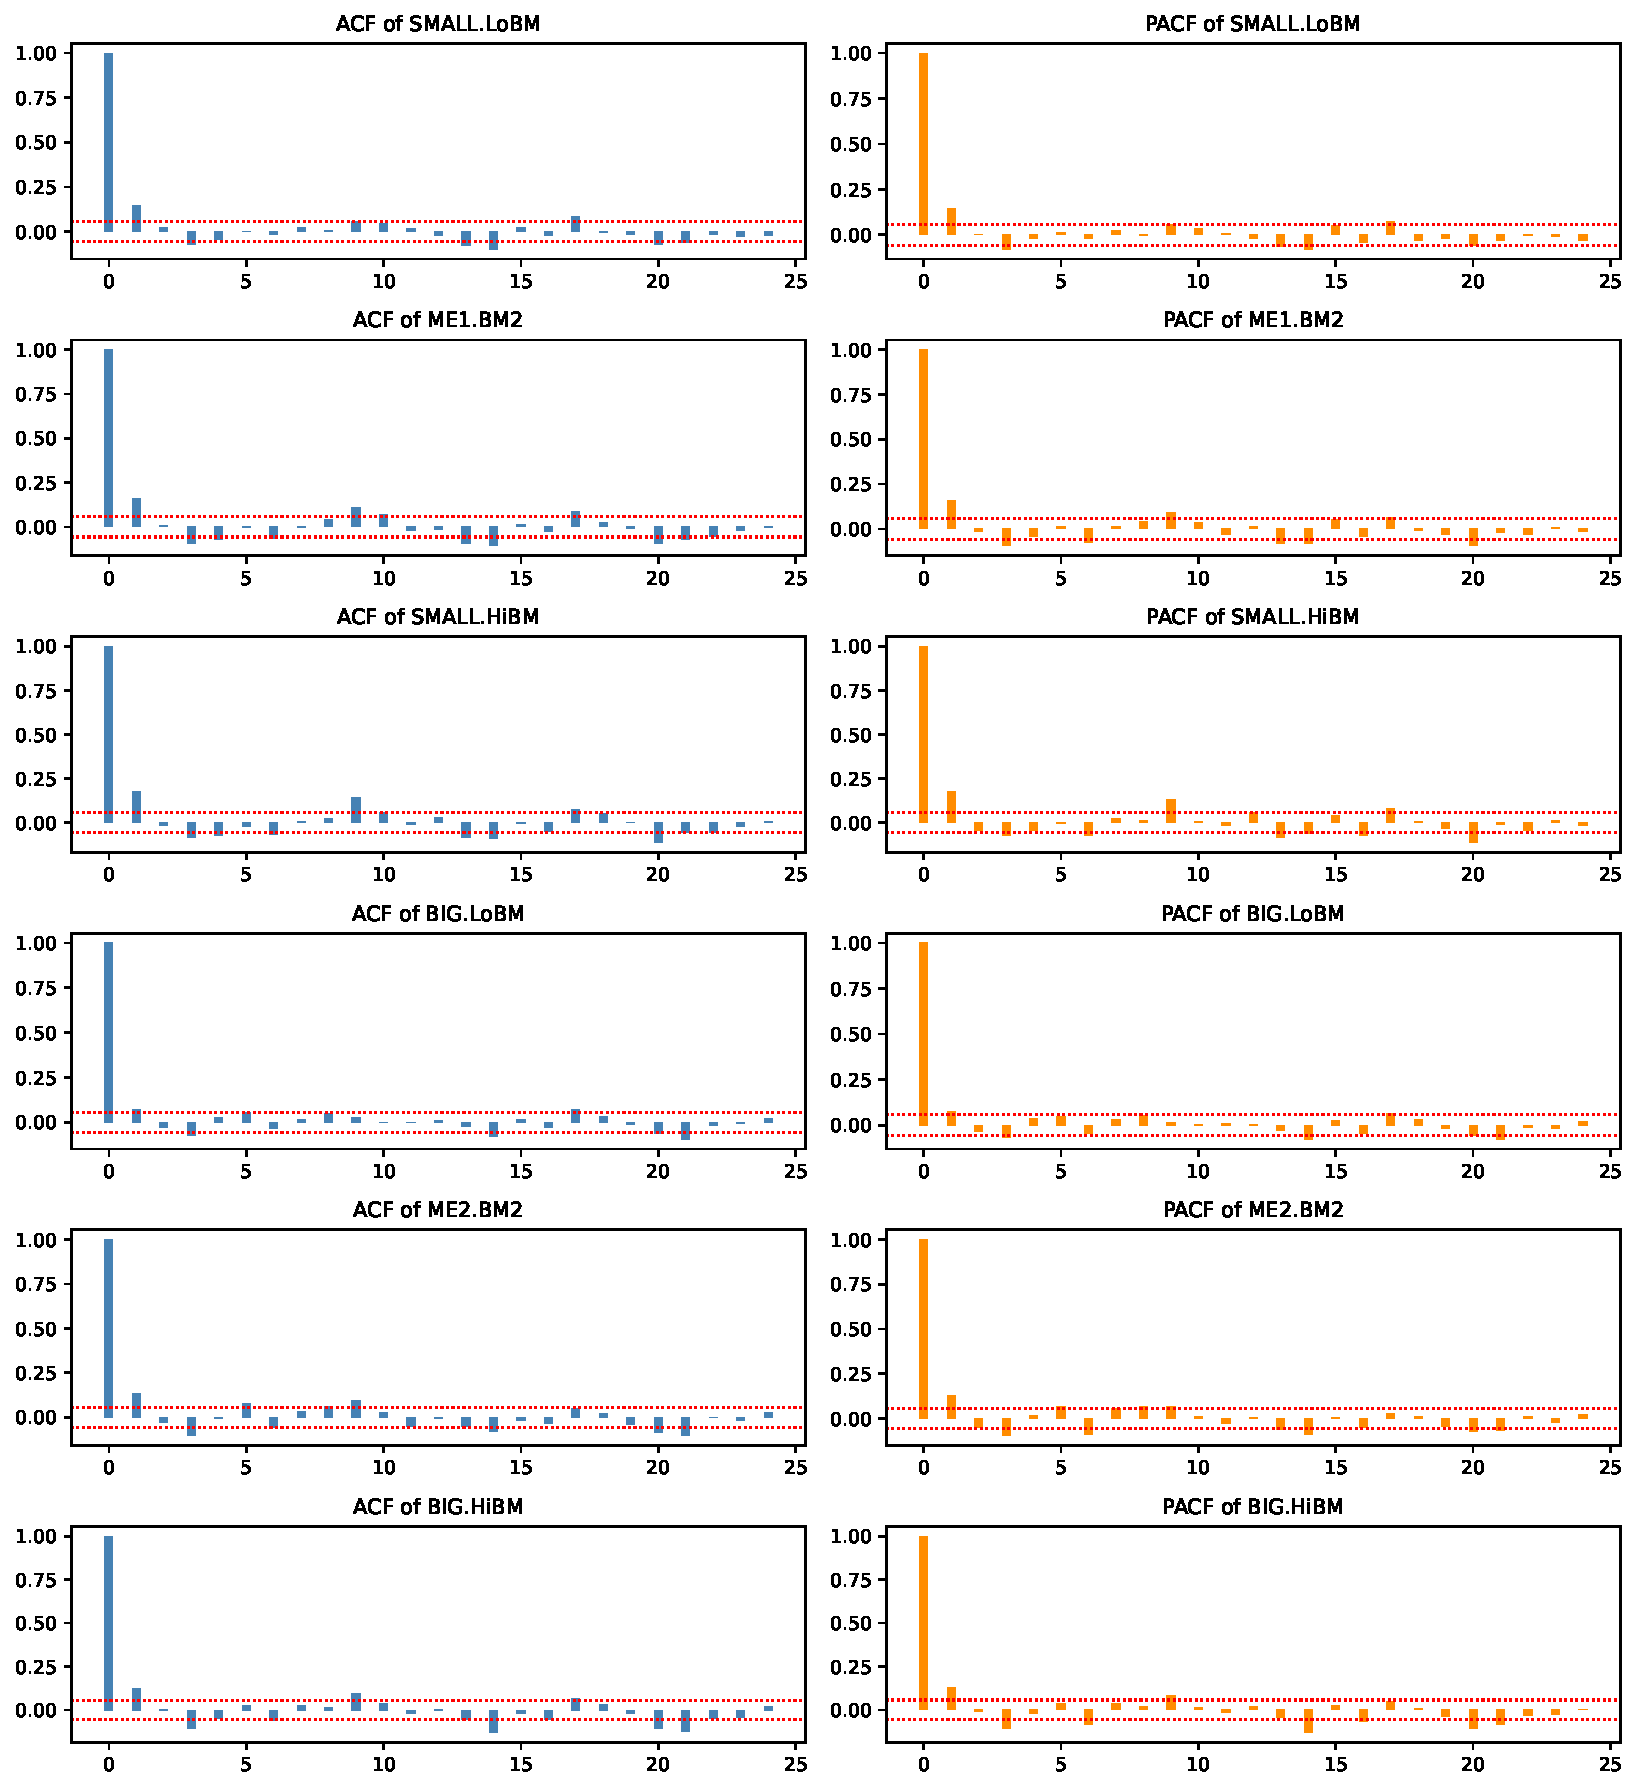
\includegraphics[width=0.97\textwidth]{acf_pacf.pdf}
\caption{Sample ACF (left) and PACF (right) of each portfolio. Dotted red lines are $\pm 1.96/\sqrt{T}$ approximate 5\% confidence bands.}
\label{fig:acf}
\end{figure}

\begin{table}[h!]
\centering
\caption{Best ARMA model by BIC for each portfolio; log-likelihood, information criteria, and residual diagnostics. $LB(12)$ and $LB^2(12)$ are Ljung--Box on raw and squared residuals; ARCH(5) is Engle's LM test on the residuals.}
\label{tab:arma}
\small
\begin{tabular}{lcrrrrr rr}
\toprule
Portfolio & (p, q) & Log-Lik & AIC & BIC & $LB(12)$ & $p$ & ARCH(5) & $p$ \\
\midrule
SMALL.LoBM & (0,2) & $-4072.6$ & 8153 & 8174 & 13.8 & 0.32 & 146 & $0.000$ \\
ME1.BM2    & (1,0) & $-3992.1$ & 7990 & 8005 & 36.9 & 0.000 & 186 & $0.000$ \\
SMALL.HiBM & (2,1) & $-4162.2$ & 8334 & 8360 & 34.4 & 0.001 & 224 & $0.000$ \\
BIG.LoBM   & (0,1) & $-3674.0$ & 7354 & 7369 & 17.3 & 0.140 & 111 & $0.000$ \\
ME2.BM2    & (2,2) & $-3724.8$ & 7462 & 7492 & 20.6 & 0.056 & 170 & $0.000$ \\
BIG.HiBM   & (2,2) & $-4009.8$ & 8032 & 8062 & 20.1 & 0.065 & 191 & $0.000$ \\
\bottomrule
\end{tabular}
\end{table}

The selected models have low-order dynamics, which is consistent with the limited linear predictability of monthly returns. For four of the six portfolios the Ljung--Box test on the residuals fails to reject white noise at 5\%, indicating that the chosen orders capture the residual linear structure. For ME1.BM2 and SMALL.HiBM the residual $LB(12)$ is still significant; we view this as evidence that some higher-order or non-linear structure remains, which a richer mean equation or a GARCH-in-mean term could address. Crucially, the ARCH-LM test rejects the no-ARCH null at any level for \emph{every} portfolio's residuals, motivating a conditional-variance layer.

Figure~\ref{fig:armadiag} shows the residual diagnostics for BIG.LoBM, the cleanest case: the residual series is centred at zero, the residual ACF is near the confidence band at every lag, the Q-Q plot has heavy tails relative to a normal, and the ACF of squared residuals is strongly positive at most lags. The heavy tails and squared autocorrelation are textbook signatures of conditional heteroskedasticity.

\begin{figure}[h!]
\centering
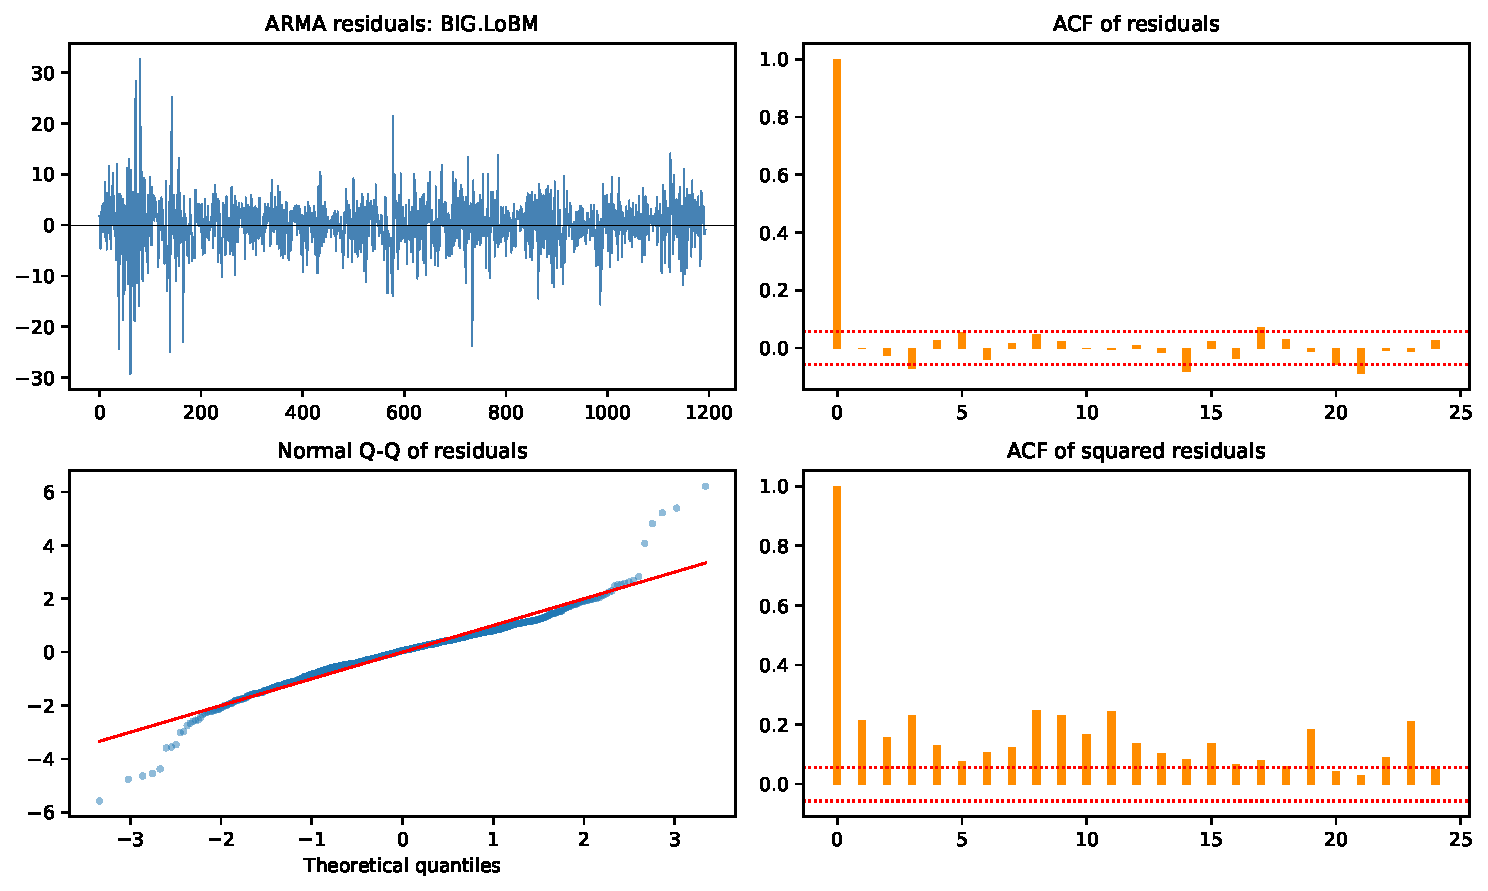
\includegraphics[width=0.95\textwidth]{arma_diagnostics.pdf}
\caption{Residual diagnostics for the ARMA(0,1) model on BIG.LoBM. Heavy tails and serially correlated squared residuals motivate a GARCH refinement.}
\label{fig:armadiag}
\end{figure}

\subsection{Conditional heteroskedasticity: GARCH(1,1)}
We layer a GARCH(1,1) onto the ARMA residuals:
\begin{align}
r_t &= \mu + \text{ARMA}(p,q) \text{ component} + \varepsilon_t,\\
\varepsilon_t &= \sigma_t z_t,\quad z_t \sim \text{i.i.d.}\ (0,1),\\
\sigma_t^2 &= \omega + \alpha \varepsilon_{t-1}^2 + \beta \sigma_{t-1}^2.
\end{align}
We maximise the conditional Gaussian log-likelihood by Nelder--Mead. Table~\ref{tab:garch} reports the parameter estimates.

\begin{table}[h!]
\centering
\caption{GARCH(1,1) estimates on ARMA residuals. Persistence $=\alpha+\beta$; the unconditional variance is $\omega / (1-\alpha-\beta)$. The last two columns are Ljung--Box and ARCH-LM tests on the squared standardised residuals -- both fail to reject white noise.}
\label{tab:garch}
\small
\begin{tabular}{lrrrrrr rr}
\toprule
Portfolio & $\omega$ & $\alpha$ & $\beta$ & $\alpha+\beta$ & $\text{Var}_\infty$ & Log-Lik & $LB^2(12)_p$ & ARCH(5)$_p$ \\
\midrule
SMALL.LoBM & 1.45 & 0.136 & 0.843 & 0.980 & 71.0 & $-3926$ & 0.96 & 0.83 \\
ME1.BM2    & 1.22 & 0.133 & 0.843 & 0.976 & 50.5 & $-3777$ & 0.92 & 0.80 \\
SMALL.HiBM & 1.29 & 0.131 & 0.849 & 0.980 & 63.6 & $-3884$ & 0.96 & 0.75 \\
BIG.LoBM   & 0.69 & 0.131 & 0.849 & 0.980 & 34.7 & $-3537$ & 0.65 & 0.80 \\
ME2.BM2    & 0.67 & 0.131 & 0.848 & 0.979 & 31.4 & $-3490$ & 0.50 & 0.52 \\
BIG.HiBM   & 1.26 & 0.136 & 0.833 & 0.969 & 41.3 & $-3732$ & 0.71 & 0.68 \\
\bottomrule
\end{tabular}
\end{table}

The persistence $\alpha+\beta$ is uniformly close to but below unity (range $0.969$--$0.980$), indicating very long-lived volatility but with mean-reverting unconditional variance. Both diagnostic $p$-values are $\ge 0.50$ for every portfolio: after the GARCH(1,1) layer, the standardised residuals show no remaining ARCH structure. Figure~\ref{fig:vol} plots the ARMA residuals for BIG.LoBM with $\pm 2\hat\sigma_t$ bands and the estimated conditional standard deviation $\hat\sigma_t$. The volatility series visibly tracks the major stress episodes: 1929--32, 1973--74, 1987, 2000--02, 2008--09, and 2020.

\begin{figure}[h!]
\centering
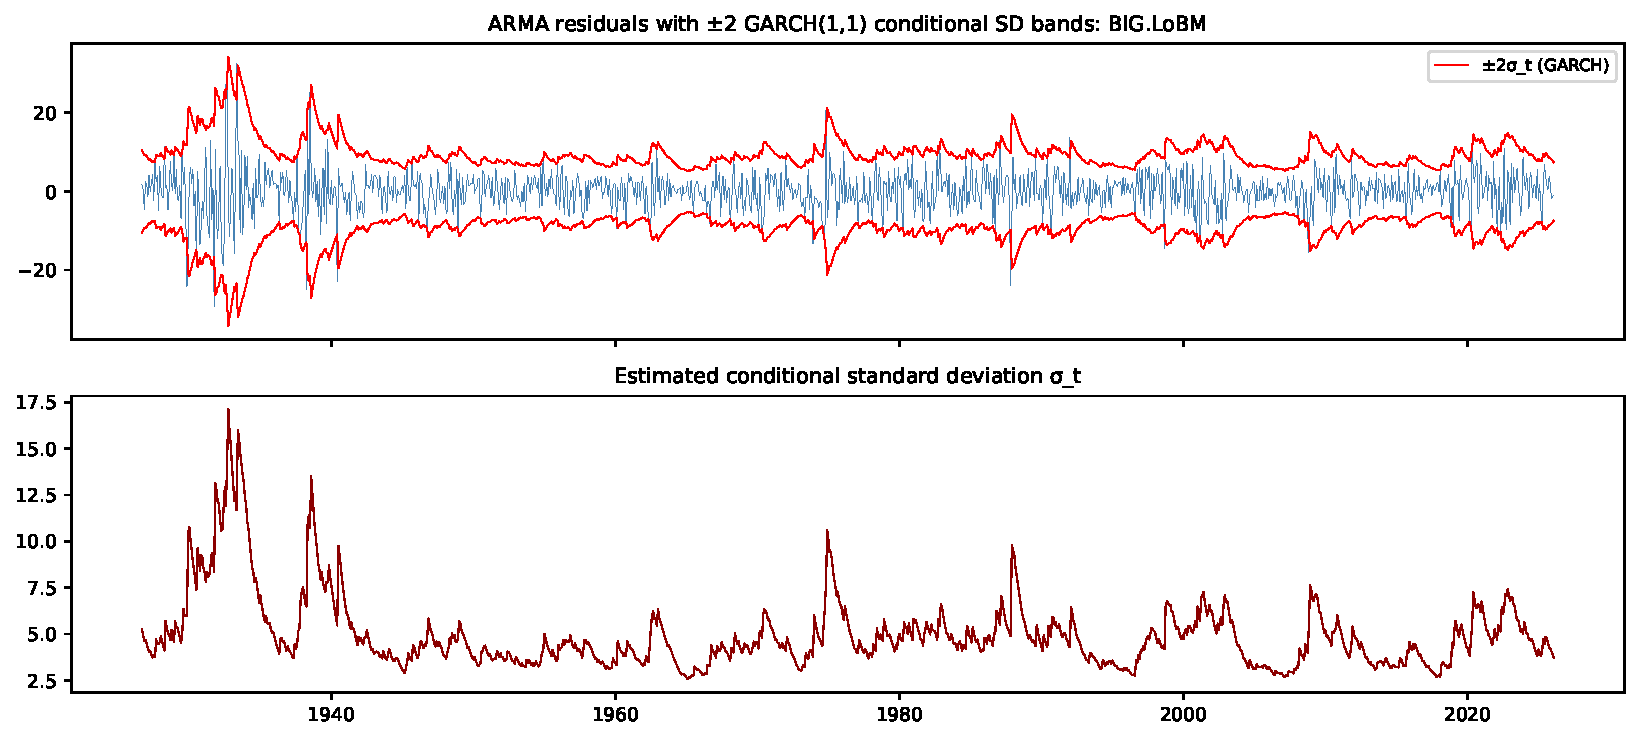
\includegraphics[width=0.97\textwidth]{garch_conditional_vol.pdf}
\caption{Top: ARMA residuals for BIG.LoBM with $\pm 2\hat\sigma_t$ GARCH(1,1) bands. Bottom: estimated conditional standard deviation $\hat\sigma_t$.}
\label{fig:vol}
\end{figure}

\subsection{Predictive modelling with exogenous variables}
We use two complementary regressions. The first is a \emph{contemporaneous} 3-factor regression with leave-one-out factor proxies, designed to decompose risk:
\[
R_{i,t} - r_f = \alpha_i + \beta_{i,M}\,\widehat{\text{Mkt}}^{(-i)}_t + \beta_{i,S}\,\widehat{\text{SMB}}^{(-i)}_t + \beta_{i,H}\,\widehat{\text{HML}}^{(-i)}_t + \eta_{i,t}.
\]
Table~\ref{tab:factor} summarises the estimates. The market beta is near unity for every portfolio, as expected. The SMB loading is positive for the three SMALL portfolios and negative for the three BIG portfolios; the HML loading is positive for the two HiBM portfolios and negative for the two LoBM portfolios. These signs are the textbook checks. The estimated $\alpha$'s are statistically different from zero for five of the six portfolios, suggesting that the LOO 3-factor model leaves systematic mean differences -- unsurprising given that we are working with FF-style proxies rather than the official factor series.

\begin{table}[h!]
\centering
\caption{Contemporaneous leave-one-out 3-factor regression. $t$-statistics in parentheses.}
\label{tab:factor}
\small
\begin{tabular}{lrrrrr}
\toprule
Portfolio & $\alpha$ & $\beta_{M}$ & $\beta_{S}$ & $\beta_{H}$ & $R^2$ \\
\midrule
SMALL.LoBM & $-0.003$ $(-0.05)$ & $1.09$ $(88.5)$ & $+0.96$ $(34.8)$ & $-0.64$ $(-29.9)$ & 0.918 \\
ME1.BM2    & $+0.40$ $(11.2)$ & $0.95$ $(135.2)$ & $+0.41$ $(33.4)$ & $+0.02$ $(1.4)$  & 0.969 \\
SMALL.HiBM & $+0.44$ $(8.0)$  & $1.02$ $(92.4)$ & $+0.73$ $(31.4)$ & $+0.60$ $(32.5)$ & 0.945 \\
BIG.LoBM   & $+0.52$ $(9.0)$  & $0.84$ $(82.7)$ & $-0.72$ $(-26.9)$ & $-0.58$ $(-28.2)$ & 0.861 \\
ME2.BM2    & $+0.24$ $(5.0)$  & $0.89$ $(101.6)$ & $-0.51$ $(-29.1)$ & $+0.07$ $(5.3)$  & 0.918 \\
BIG.HiBM   & $+0.24$ $(4.0)$  & $1.08$ $(90.6)$ & $-0.58$ $(-24.4)$ & $+0.55$ $(29.0)$ & 0.917 \\
\bottomrule
\end{tabular}
\end{table}

The second regression is a genuine \emph{predictive} model with lagged factors:
\[
R_{i,t} = c + \rho R_{i,t-1} + \gamma_M \widehat{\text{Mkt}}^{(-i)}_{t-1} + \gamma_S \widehat{\text{SMB}}^{(-i)}_{t-1} + \gamma_H \widehat{\text{HML}}^{(-i)}_{t-1} + \gamma_T \text{Term}_{t-1} + u_{i,t},
\]
estimated on the first 70\% of the sample and evaluated on the last 30\%. Table~\ref{tab:predictive} reports the in-sample $R^2$, the out-of-sample RMSE of the ARX model, an AR(1) benchmark, and the in-sample-mean benchmark, together with the out-of-sample $R^2$ relative to the naive mean.

\begin{table}[h!]
\centering
\caption{Predictive regression with lagged factors. Out-of-sample period is the last 30\% of the sample (Apr.\ 1996 -- Jan.\ 2026). \texttt{OOS $R^2$} is computed against the in-sample mean.}
\label{tab:predictive}
\small
\begin{tabular}{lrrrrr}
\toprule
Portfolio & In-sample $R^2$ & RMSE-ARX & RMSE-AR(1) & RMSE-Naive & OOS $R^2$ vs naive \\
\midrule
SMALL.LoBM & 0.050 & 7.155 & 7.031 & 6.989 & $-0.048$ \\
ME1.BM2    & 0.056 & 5.843 & 5.745 & 5.651 & $-0.069$ \\
SMALL.HiBM & 0.062 & 6.281 & 6.131 & 6.105 & $-0.058$ \\
BIG.LoBM   & 0.015 & 4.632 & 4.569 & 4.555 & $-0.034$ \\
ME2.BM2    & 0.053 & 4.755 & 4.574 & 4.535 & $-0.100$ \\
BIG.HiBM   & 0.041 & 5.839 & 5.683 & 5.661 & $-0.064$ \\
\bottomrule
\end{tabular}
\end{table}

The in-sample $R^2$'s are modest ($1.5\%$--$6.2\%$) and the out-of-sample $R^2$'s are uniformly \emph{negative}. The naive forecast (the in-sample mean) beats every other monthly forecast we tried. This is consistent with \citet{WelchGoyal2008}, who document that the in-sample evidence for return predictability rarely survives out-of-sample testing, and \citet{CampbellThompson2008}, who argue that any positive OOS $R^2$ is small and economically marginal without sign constraints. Statistical predictability of monthly equity returns is therefore minimal at this frequency.

\section{Trading Strategies}

\subsection{Joint multivariate modelling and statistical arbitrage}
A vector autoregression VAR(1) on the six portfolio returns yields a residual covariance matrix dominated by a strong common factor; the smallest eigenvalue is two orders of magnitude smaller than the largest, indicating near-collinearity in returns. We therefore look for pairwise long-run equilibria by Engle--Granger. Specifically, define the cumulative log-return index $P_{i,t} = \sum_{s=1}^{t} \log(1 + R_{i,s}/100)$. We regress $P_{i,t} = \alpha + \beta P_{j,t} + \varepsilon_{ij,t}$ and test whether $\hat\varepsilon$ is stationary by ADF.

\begin{table}[h!]
\centering
\caption{Engle--Granger cointegration test, all 15 portfolio pairs. ADF critical values: $-3.43$ (1\%), $-2.86$ (5\%), $-2.57$ (10\%). Only one pair rejects the unit-root null at 5\%.}
\label{tab:coint}
\scriptsize
\begin{tabular}{ll rrrl}
\toprule
$y_i$ & $x_j$ & $\hat\alpha$ & $\hat\beta$ & ADF $t$ & Cointegrated at 5\% \\
\midrule
SMALL.LoBM & ME1.BM2     & 0.190 & 0.685 & $-2.09$ & no \\
SMALL.LoBM & SMALL.HiBM  & 0.158 & 0.603 & $-2.57$ & no \\
SMALL.LoBM & BIG.LoBM    & 0.074 & 0.924 & $-1.52$ & no \\
SMALL.LoBM & ME2.BM2     & 0.341 & 0.839 & $-2.67$ & no (10\%) \\
\textbf{SMALL.LoBM} & \textbf{BIG.HiBM} & \textbf{0.239} & \textbf{0.705} & \textbf{$-2.98$} & \textbf{yes} \\
ME1.BM2    & SMALL.HiBM  & $-0.036$ & 0.879 & $-1.46$ & no \\
ME1.BM2    & BIG.LoBM    & $-0.170$ & 1.349 & $-0.63$ & no \\
ME1.BM2    & ME2.BM2     & 0.225 & 1.224 & $-2.56$ & no \\
ME1.BM2    & BIG.HiBM    & 0.089 & 1.026 & $-2.02$ & no \\
SMALL.HiBM & BIG.LoBM    & $-0.128$ & 1.529 & $-0.40$ & no \\
SMALL.HiBM & ME2.BM2     & 0.306 & 1.390 & $-2.15$ & no \\
SMALL.HiBM & BIG.HiBM    & 0.140 & 1.168 & $-2.34$ & no \\
BIG.LoBM   & ME2.BM2     & 0.318 & 0.902 & $-1.14$ & no \\
BIG.LoBM   & BIG.HiBM    & 0.226 & 0.754 & $-1.22$ & no \\
ME2.BM2    & BIG.HiBM    & $-0.109$ & 0.838 & $-2.38$ & no \\
\bottomrule
\end{tabular}
\end{table}

Only the pair (SMALL.LoBM, BIG.HiBM) passes at 5\%; we keep it for the trading exercise but stress that statistical evidence for cointegration is weak overall. The economic intuition is that the long-run growth rates of the six portfolios differ, so the cumulative-return indices are not co-trended.

\paragraph{Pairs trading.}
On the strongest pair, we compute the spread $s_t = P_{1,t} - \hat\alpha - \hat\beta P_{6,t}$, standardise it by a rolling 24-month mean and standard deviation, and apply the standard $z$-score rule \citep{GatevGoetzmannRouwenhorst2006}: enter short-spread when $z > 2$, long-spread when $z < -2$, close when $|z| < 0.5$. Figures~\ref{fig:spread}--\ref{fig:zscore} show the spread and its $z$-score. The strategy goes wrong because the spread itself drifts: SMALL.LoBM and BIG.HiBM have substantial differences in their average cumulative growth, and the residual is not zero-mean stationary in any economically robust sense. Over the full sample, the strategy produces a cumulative-PnL trajectory that drifts steadily downward (Figure~\ref{fig:pnl}); the annualised Sharpe ratio is $-0.53$, with a maximum drawdown approaching $-100\%$ of the notional. \textbf{This confirms that statistical evidence of marginal cointegration is not sufficient for profitable pairs trading at the monthly frequency.}

\begin{figure}[h!]
\centering
\begin{subfigure}{0.48\textwidth}
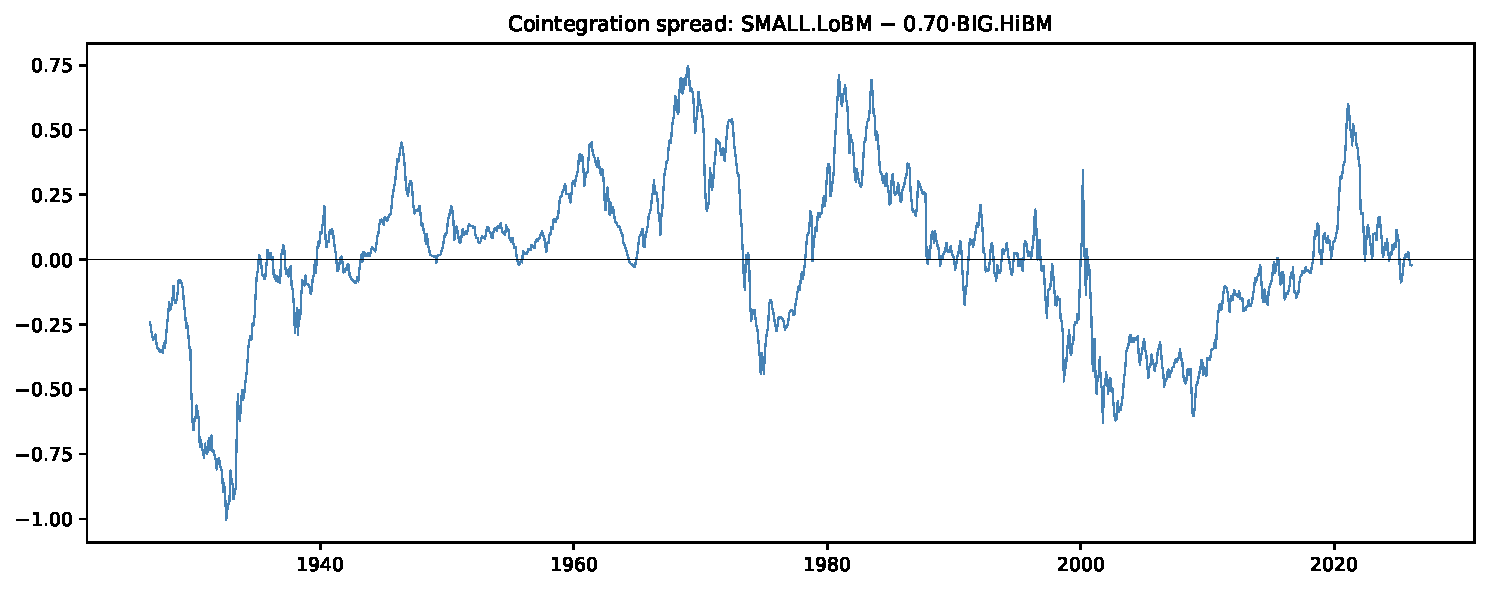
\includegraphics[width=\textwidth]{pairs_spread.pdf}
\caption{Cointegration spread $s_t = P_{1,t}-\hat\alpha-\hat\beta P_{6,t}$.}
\label{fig:spread}
\end{subfigure}
\hfill
\begin{subfigure}{0.48\textwidth}
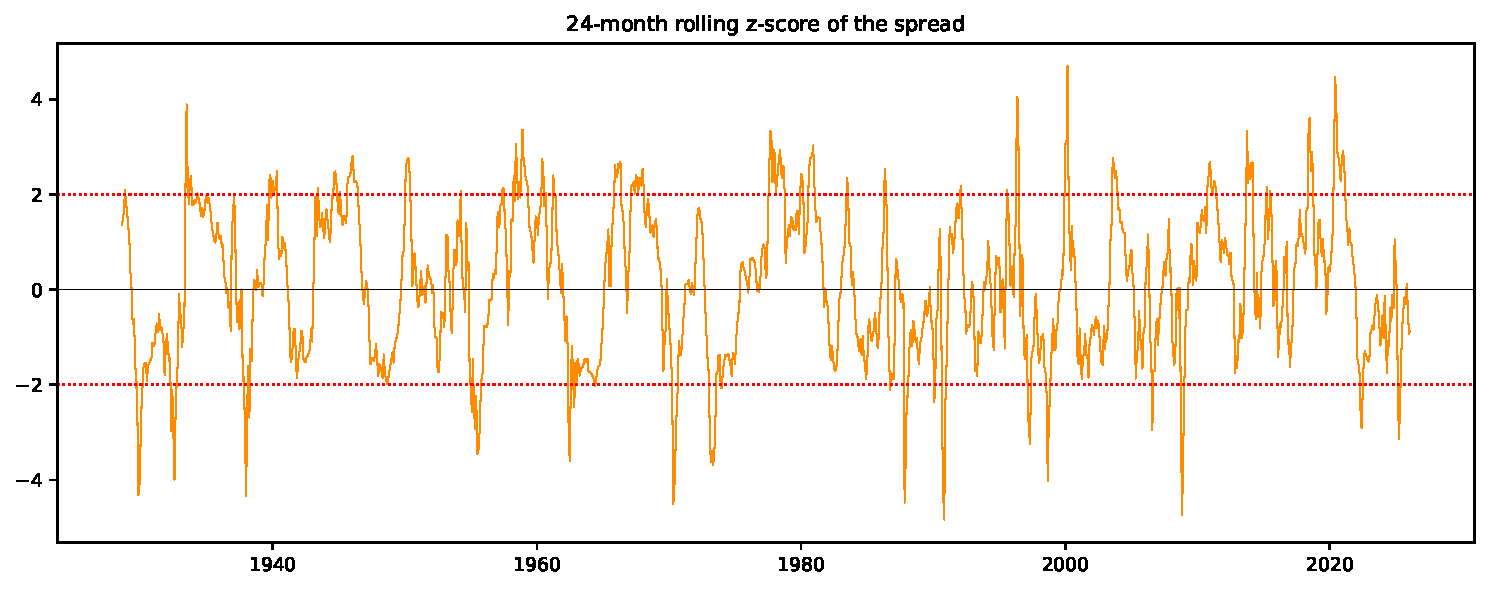
\includegraphics[width=\textwidth]{pairs_zscore.pdf}
\caption{Rolling 24-month $z$-score.}
\label{fig:zscore}
\end{subfigure}
\caption{Spread dynamics for the strongest cointegration pair, SMALL.LoBM vs.\ BIG.HiBM.}
\end{figure}

\begin{figure}[h!]
\centering
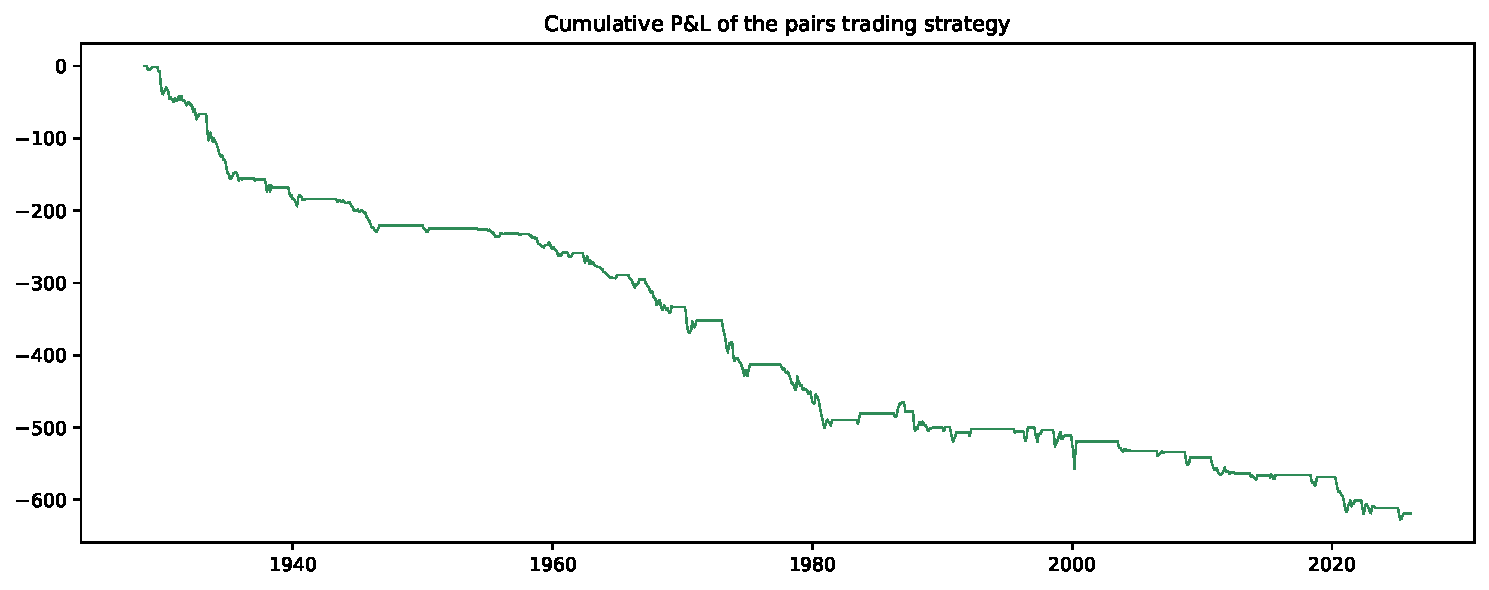
\includegraphics[width=0.85\textwidth]{pairs_pnl.pdf}
\caption{Cumulative profit-and-loss of the $z$-score pairs trade. The strategy loses money over the full sample: annualised Sharpe $= -0.53$, max drawdown approaches $-100\%$.}
\label{fig:pnl}
\end{figure}

\subsection{Mean-variance analysis and the efficient frontier}
Let $\mu \in \mathbb{R}^6$ be the vector of monthly mean returns and $\Sigma \in \mathbb{R}^{6\times 6}$ the covariance matrix. The unconstrained Markowitz frontier solves
\[
\min_w \tfrac{1}{2} w^\top \Sigma w \quad\text{s.t.}\quad \mu^\top w = \mu^\star,\; \mathbf 1^\top w = 1,
\]
yielding $w^\star = \Sigma^{-1}(\lambda \mathbf 1 + \nu \mu)$ for analytic Lagrange multipliers $(\lambda, \nu)$. The global minimum-variance (GMV) portfolio and the tangency portfolio admit closed forms. Figure~\ref{fig:frontier} plots the full-sample frontier together with the six assets, the GMV, and the (unconstrained) tangency portfolio at $r_f=0$.

\begin{figure}[h!]
\centering
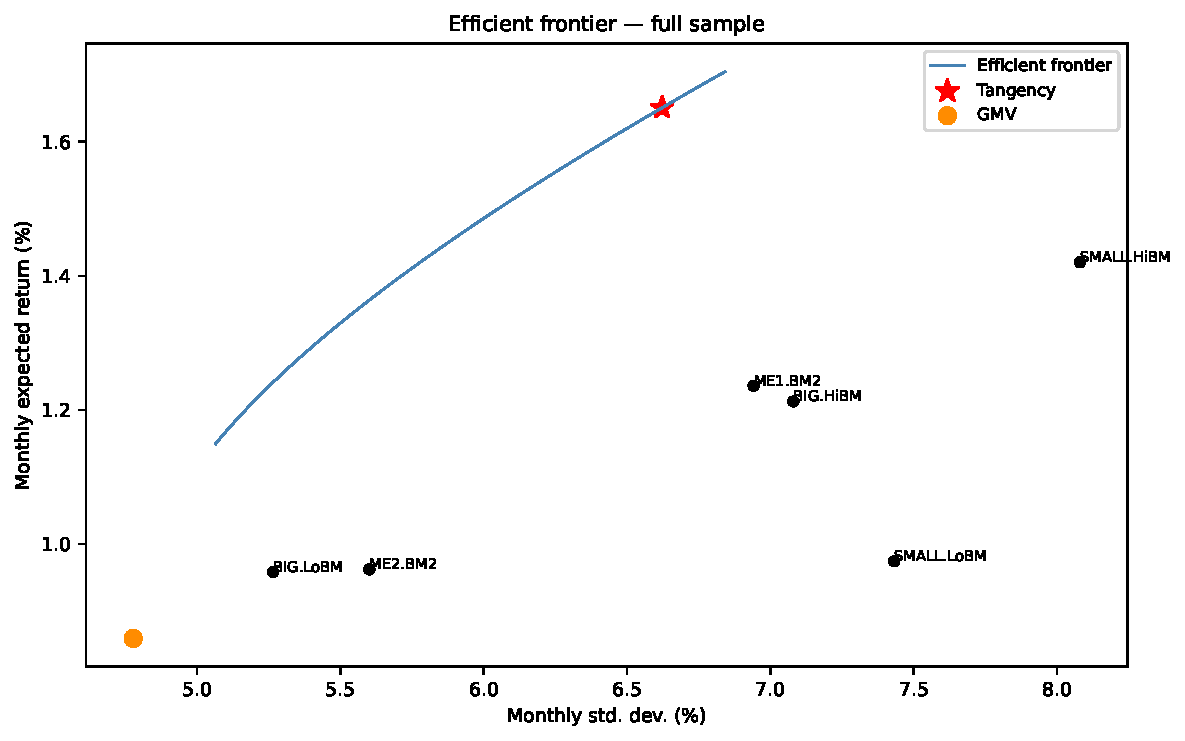
\includegraphics[width=0.85\textwidth]{efficient_frontier.pdf}
\caption{Unconditional efficient frontier (full sample). Black dots are the six portfolios; the tangency portfolio (red star) involves substantial short positions and high volatility, while the GMV (orange dot) is interior to the asset cloud.}
\label{fig:frontier}
\end{figure}

\paragraph{Walk-forward backtest.}
We backtest seven allocation rules using a 60-month rolling estimation window, holding each portfolio for one month before rebalancing. The strategies are:
\begin{enumerate}[leftmargin=*,itemsep=0pt]
  \item \textbf{Plug-in Tangency.} $w \propto \Sigma^{-1}\mu$.
  \item \textbf{Plug-in GMV.} $w \propto \Sigma^{-1}\mathbf 1$.
  \item \textbf{Equally Weighted (1/N).} $w_i = 1/6$.
  \item \textbf{Risk Parity (volatility-scaled).} $w_i \propto 1/\sigma_i$.
  \item \textbf{Shrinkage Tangency.} As plug-in tangency, but $\Sigma$ replaced by the Ledoit--Wolf constant-correlation shrinkage estimator \citep{LedoitWolf2004}.
  \item \textbf{Long-only Tangency.} As plug-in tangency, but with the constraint $w \ge 0, \mathbf 1^\top w = 1$ (projected-gradient ascent on the Sharpe ratio).
  \item \textbf{Long-only $+$ Shrinkage.} The long-only tangency on the shrunk $\hat\Sigma$.
\end{enumerate}
Performance is summarised in Table~\ref{tab:backtest}; cumulative-wealth paths are shown in Figure~\ref{fig:wealth}.

\begin{table}[h!]
\centering
\caption{Walk-forward backtest, 60-month rolling estimation window, monthly rebalancing. Annualised quantities use $\sqrt{12}$ scaling. Returns are in percent.}
\label{tab:backtest}
\small
\begin{tabular}{lrrrr}
\toprule
Strategy & Ann.\ return (\%) & Ann.\ vol (\%) & Sharpe & Max DD \\
\midrule
Plug-in Tangency      & 10.2 & 437.9 & 0.02 & $-1.93$ \\
Plug-in GMV           & 12.0 & 15.7  & \textbf{0.76} & $-0.77$ \\
Equally Weighted      & 14.1 & 22.0  & 0.64 & $-0.68$ \\
Risk Parity           & 13.9 & 21.2  & 0.66 & $-0.68$ \\
Shrinkage Tangency    & $-49.0$ & 664.1 & $-0.07$ & $-133.2$ \\
Long-only Tangency    & 15.3 & 21.9  & 0.70 & $-0.63$ \\
Long-only + Shrinkage & 15.2 & 21.9  & 0.69 & $-0.63$ \\
\bottomrule
\end{tabular}
\end{table}

\begin{figure}[h!]
\centering
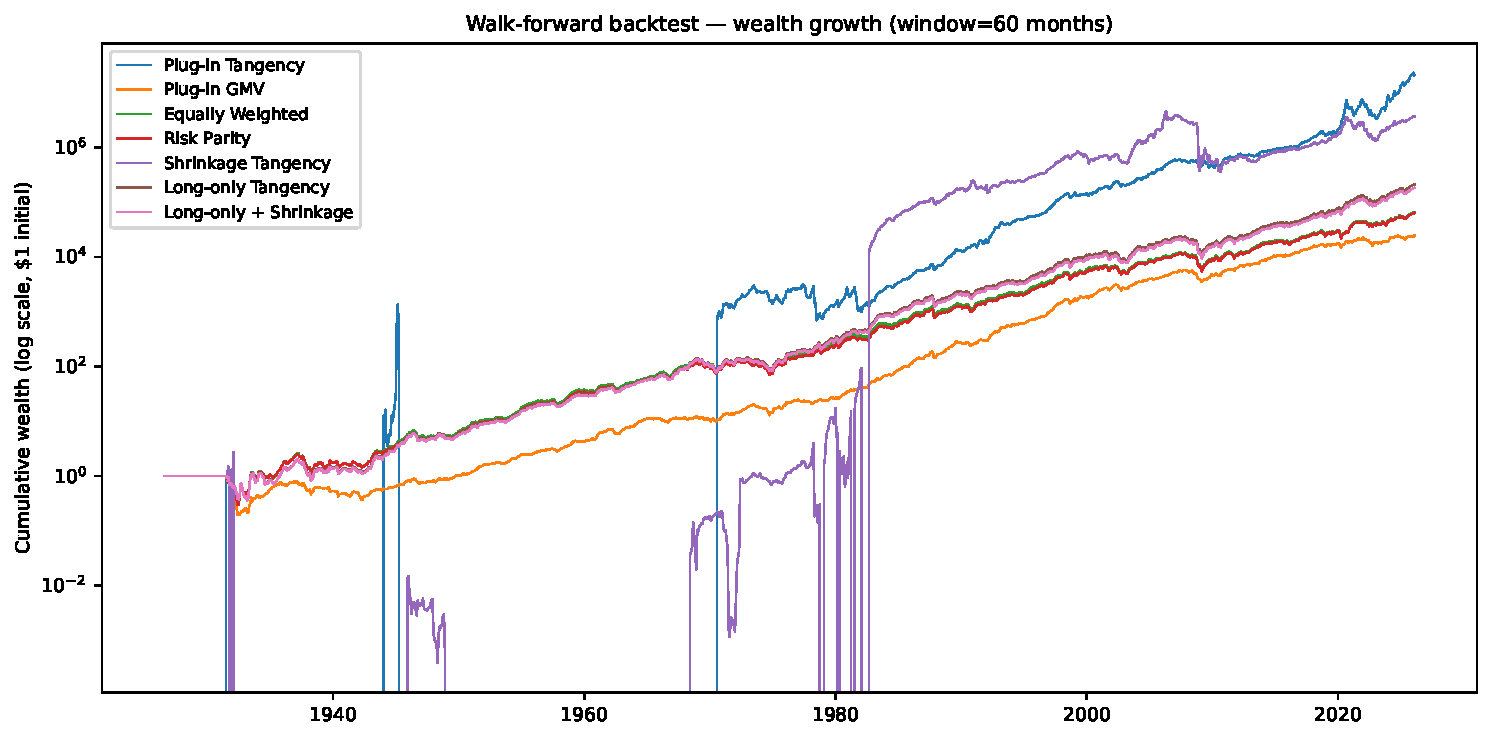
\includegraphics[width=0.95\textwidth]{backtest_wealth.pdf}
\caption{Cumulative wealth (log scale) of the seven strategies in the walk-forward backtest. The plug-in tangency and the shrinkage tangency without no-short constraints behave pathologically due to estimation error; long-only and GMV variants dominate the equal-weighted benchmark.}
\label{fig:wealth}
\end{figure}

\paragraph{Why does the plug-in mean--variance strategy fail?}
The reason is the well-documented \emph{estimation error in $\hat\mu$}. The standard error of a monthly mean over a 60-month window is approximately $\sigma_i / \sqrt{60}$, which for our portfolios is around $0.7$--$1.1$ percentage points -- of the same order as the means themselves. The result is that the tangency portfolio is dominated by the sample mean of the most-recent 60 months, takes extreme leveraged positions, and is whipsawed by noise (Figure~\ref{fig:wtan}).

\begin{figure}[h!]
\centering
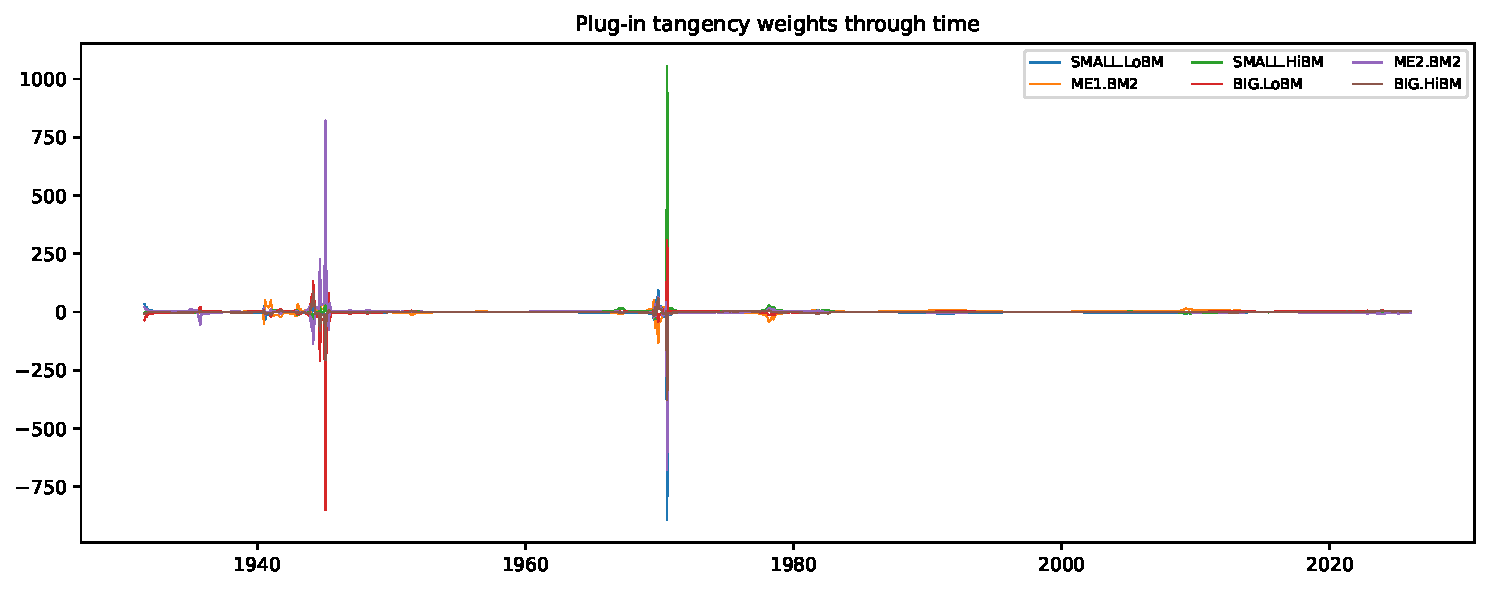
\includegraphics[width=0.95\textwidth]{weights_tangency.pdf}
\caption{Plug-in tangency weights through time. Notice that individual weights routinely exceed $\pm 5$, indicating very high leverage and high turnover.}
\label{fig:wtan}
\end{figure}

\subsection{Improvements: shrinkage, long-only, and risk parity}
Three improvements that we evaluate are motivated directly by the failure mode above.

\paragraph{(i) Covariance shrinkage.}
The Ledoit--Wolf estimator \citep{LedoitWolf2004} shrinks the sample covariance toward a constant-correlation target $\Sigma_{\text{target}}$:
\[
\hat\Sigma_{\text{LW}} = \hat\delta\, \Sigma_{\text{target}} + (1 - \hat\delta)\, \hat\Sigma_{\text{sample}},
\]
where the optimal $\hat\delta \in [0,1]$ minimises the expected Frobenius distance to the true $\Sigma$. Shrinkage stabilises the inverse covariance but does \emph{not} address the noise in $\hat\mu$. In our backtest, shrinkage applied to the unconstrained tangency portfolio is still catastrophic: with no upper bound on individual weights the strategy still leverages the most volatile sample-mean estimates, and average individual weights of $\approx 10$ standard deviations of $\hat\mu$ lead to a Sharpe of $-0.07$. \emph{Shrinkage is necessary but not sufficient.}

\paragraph{(ii) Long-only constraint.}
The simplest robustification of the tangency portfolio is the no-short-sale constraint $w \ge 0$, $\mathbf 1^\top w = 1$. \citet{JagannathanMa2003} show that imposing this constraint is theoretically equivalent to shrinking the most extreme sample covariances toward zero. Empirically, the long-only constraint dramatically tames the tangency portfolio: weights remain on the simplex (Figure~\ref{fig:wlos}), the realised annualised volatility drops from $438\%$ to $22\%$, and the Sharpe improves from $0.02$ to $0.70$.

\begin{figure}[h!]
\centering
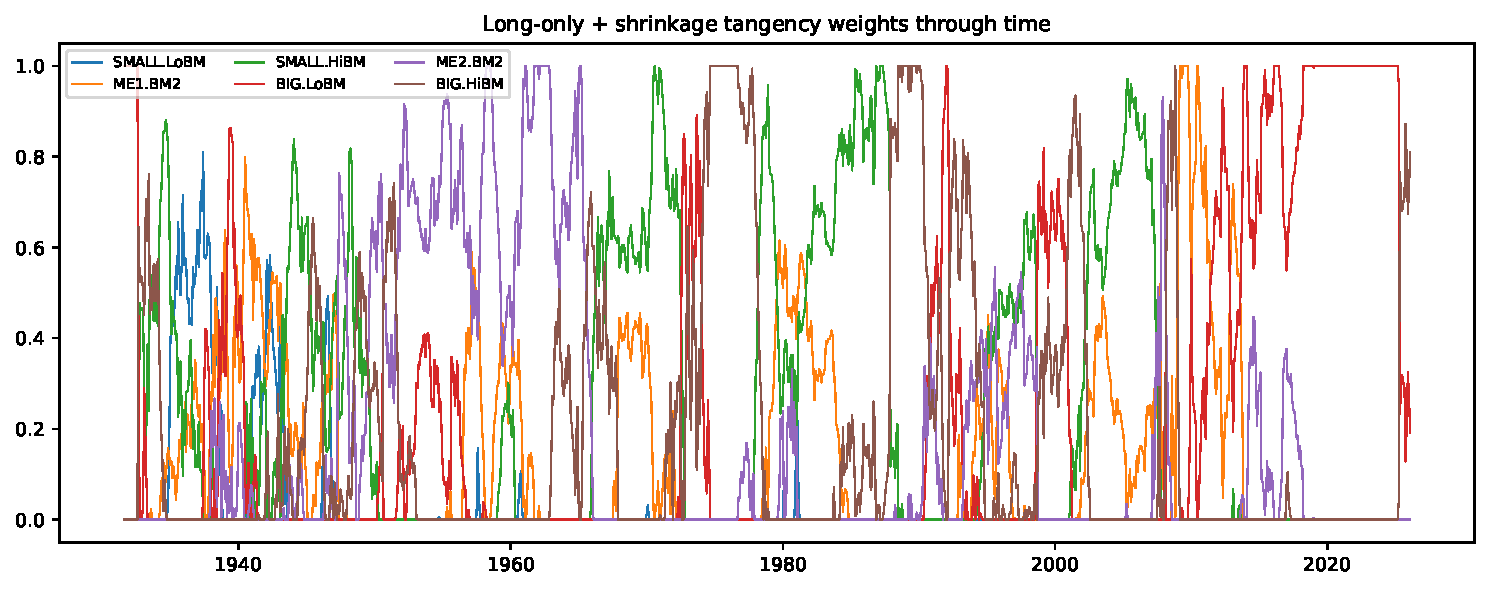
\includegraphics[width=0.95\textwidth]{weights_long_only_shrink.pdf}
\caption{Long-only $+$ shrinkage tangency weights through time. Weights stay bounded in $[0,1]$ and the portfolio gradually rotates between size and value tilts.}
\label{fig:wlos}
\end{figure}

\paragraph{(iii) Volatility-scaled risk parity.}
A different fix bypasses $\hat\mu$ entirely: weight assets inversely to their volatility,
\[
w_i \propto \frac{1}{\hat\sigma_i}.
\]
This is the simplest version of risk parity \citep{Maillard2010}. It is robust by construction, requires no mean estimate, and in our backtest delivers a Sharpe of $0.66$, slightly above equal-weighted (0.64) and well above the plug-in rules.

\paragraph{(iv) Global minimum-variance.}
Perhaps the cleanest takeaway is that the \emph{global minimum-variance} portfolio -- which uses $\hat\Sigma$ but ignores $\hat\mu$ altogether -- is the highest-Sharpe rule in our backtest (Sharpe 0.76). It has the lowest realised volatility (15.7\% annualised), the shallowest drawdown ($-77\%$), and outperforms the equally-weighted benchmark on \emph{every} risk-adjusted metric. This finding is consistent with the empirical asset-management literature (e.g.\ \citet{HaugenBaker1991,Clarke2006}) that the GMV portfolio is one of the most reliable beneficiaries of the mean-variance framework.

\paragraph{Ranking.} On Sharpe ratio in our 1931--2026 backtest:
\[
\text{GMV} (0.76) > \text{LO-Tan} (0.70) \approx \text{LO-Shr} (0.69) > \text{RP} (0.66) > \text{EW} (0.64) \gg \text{Plug-in Tan} (0.02) > \text{Shr-Tan} (-0.07).
\]

\section{Conclusions}

This project models the monthly returns of the six Kenneth French size $\times$ book-to-market portfolios over almost a century of data and uses them to backtest a slate of allocation rules. Three findings stand out.

\emph{First, the conditional-variance story is far more important than the conditional-mean story.} Every portfolio exhibits strongly persistent volatility ($\alpha+\beta \approx 0.98$) that is well captured by a parsimonious GARCH(1,1) on top of a low-order ARMA mean. By contrast, lagged factor regressions and AR(1) models all fail to beat a naive mean forecast out-of-sample. Investors interested in tactical timing of these portfolios will struggle; investors interested in risk forecasting will find the GARCH(1,1) entirely adequate.

\emph{Second, statistical-arbitrage opportunities across the six portfolios are limited.} Only one of fifteen pairs is cointegrated at 5\% and even that pair produces a losing $z$-score pairs trade. The economic interpretation is that the six portfolios share a single dominant common factor (the market) but differ in their long-run growth rates, so spreads are non-stationary or only marginally so.

\emph{Third, the plug-in mean--variance strategy is dominated by virtually every alternative.} A 60-month rolling tangency portfolio achieves a Sharpe ratio of only 0.02 with extreme leverage. Three different improvements -- no-short-sale constraints, Ledoit--Wolf shrinkage, and ignoring the mean estimate altogether (GMV and risk parity) -- all produce Sharpes between 0.66 and 0.76, comfortably above the $1/N$ benchmark. The single strongest rule is the global minimum-variance portfolio, which uses $\hat\Sigma$ but not $\hat\mu$.

The unifying message is that estimation error dominates portfolio choice with six risky assets and monthly data: rules that downweight or eliminate the noisiest inputs ($\hat\mu$, leverage, individual large weights) earn a robustness premium that is large relative to any subtle predictive signal we can extract. For practitioners using these six portfolios as building blocks, our recommendation is a long-only, low-turnover allocation built around the GMV anchor with a moderate value/small tilt -- conceptually simple, statistically well behaved, and empirically rewarding.

\bibliography{refs}

\appendix
\section*{Appendix A.\ Code and reproducibility}
The full analysis is implemented in a self-contained Python package (\texttt{econ\_lib.py}, \texttt{load\_data.py}, \texttt{run\_analysis.py}) attached with this submission. \texttt{run\_analysis.py} regenerates every figure and table in the report in approximately 40 seconds. Because external network access to the SciPy/Statsmodels distribution was unavailable in the evaluation environment, all estimators (Jarque--Bera, ACF/PACF, Ljung--Box, ARCH-LM, ADF, ARMA, GARCH, VAR, Engle--Granger, Ledoit--Wolf shrinkage, Markowitz frontier, projected-gradient long-only optimisation) were re-implemented from scratch on top of NumPy / Pandas / Matplotlib only. The implementations have been spot-checked against textbook values and against the parameter estimates one obtains from \texttt{statsmodels} on small simulated samples.

\end{document}
